%% updated_PAI_report.tex -- PAI Group Project, NCI MSc AI, April 2026

\documentclass[journal]{IEEEtran}
\usepackage{amsmath}
\usepackage{booktabs}
\usepackage{tikz}
\usetikzlibrary{arrows.meta,shapes.geometric,positioning}
\usepackage{pgfplots}
\pgfplotsset{compat=1.18}
\hyphenation{op-tical net-works semi-conduc-tor}

\begin{document}

\title{Multimodal Regime Adaptive Transformer and Reinforcement\\
Learning for Global Financial Forecasting}

\author{Divyesh~Reddy~Ellasiri,
        Sai~Vivek~Yerninti,
        Mukesh~Saren~Ramu,
        and~Alabi~Taiwo~Oluwatamilore%
\thanks{All authors are with the School of Computing, National College of
Ireland, Dublin, Ireland. Student IDs: 25134825, 25138286, 25121448,
24335592.}%
\thanks{Submitted in partial fulfilment of Programming for Artificial
Intelligence, MSc Artificial Intelligence, April 2026.}}

\markboth{MSc Artificial Intelligence, Programming for AI, NCI Dublin, 2026}%
{Ellasiri \MakeLowercase{\textit{et al.}}: Multimodal Regime Adaptive
Transformer and RL for Global Financial Forecasting}

\maketitle

\begin{abstract}
Global markets move faster than any human can reasonably track. Forty eight
assets across four asset classes each produce hundreds of price signals
daily. The question this project set out to answer was not whether AI can
help, but whether one fixed model type survives contact with all of them
simultaneously. This paper presents MRAT-RL, a multimodal, regime-aware
trading system combining a PatchTST Transformer, three Reinforcement
Learning agents (SAC, TD3, PPO), and Hidden Markov Model regime detection
into a single daily pipeline. Training data was sourced from four distinct
datasets: Yahoo Finance daily OHLCV prices (2004--2026), CBOE VIX
volatility indices, FRED short-term interest rate series, and a
sentiment proxy derived from Bollinger Band and volume signals; all
collected programmatically and stored in a structured SQLite database. A Deep Learning Laboratory ran 1200 training
experiments to find the best forecasting architecture per asset; CNN and
LSTM models outperformed PatchTST on 39 of 48-assets and were promoted to
production. On 9 April 2026, the system scanned 47 assets and produced 17
BUY signals, 2 SELL signals, and 28 HOLD signals at an average confidence
of 59 per cent. All detected market regimes were bullish or sideways; 5 day
return forecasts ranged from $+1.5\%$ to $-0.4\%$, consistent with
realistic short-term return distributions. Backtesting across 7800 walk
forward windows confirmed an average annual return of $+1.85\%$ per window,
a Sharpe ratio of 0.91, and a drawdown of only $-1.2\%$ during the 2022
bear market; a period when the S\&P 500 fell $-20\%$ and Bitcoin fell
$-65\%$.
\end{abstract}

\begin{IEEEkeywords}
time series forecasting, Transformer, PatchTST, reinforcement learning,
SAC, PPO, regime detection, Hidden Markov Model, portfolio optimisation,
deep learning
\end{IEEEkeywords}

\IEEEpeerreviewmaketitle

% -----------------------------------------------------------------------
\section{Introduction}
\label{sec:intro}
% -----------------------------------------------------------------------

\IEEEPARstart{F}{inancial} markets do not behave the same way twice. A
strategy earning steady returns during a quiet bull run can destroy capital
in three sessions once volatility spikes. A model trained on calm data has
never seen what fear looks like on a price chart; a model trained solely
on crash data grows paralysed whenever nothing dramatic happens. This
tension, between pattern and regime, between order and chaos, defines the
central challenge every serious algorithmic trading system must solve.

Traditional forecasting tools treat markets as stationary: the
relationship between inputs and outputs stays fixed over time. Linear
regression, ARIMA, and basic moving average crossovers all share this
assumption. Markets violate it constantly. From March 2020 to November
2021, equities entered one of the fastest recoveries ever recorded. From
January 2022, those same assets shed a third of their value across nine
months. No fixed-rule model navigates both regimes correctly; the rules
that worked in one world fail in the other.

Deep learning changed what became possible. Neural networks learn
nonlinear patterns directly from data, without hand-crafted rules and
without stationarity assumptions. Transformer-based architectures
\cite{informer,autoformer,tft} showed that attention mechanisms,
originally designed for natural language, generalise remarkably well to
time series data. PatchTST \cite{patchtst} pushed this further; rather
than treating each daily close as a separate token, it groups consecutive
days into patches and attends across them, capturing short-term momentum
and long-range structural patterns within a single forward pass.

Reinforcement Learning adds a different dimension entirely. A forecasting
model predicts prices; an RL agent decides what to do about them
\cite{sarl,stockformer}. The distinction matters more than it first
appears. A model can be directionally correct and still lose money,
entering too early, sizing too large, or holding past the point where
conditions changed. RL agents learn \emph{when} to act, not just what
tomorrow's price might be.

Most published systems stop at one asset class or one model type. Real
portfolios do not. Equities, cryptocurrencies, foreign exchange, and
commodities coexist within any serious portfolio, each behaving
differently. Cryptocurrencies can move ten times as fast as equities
across a single volatile day. Forex pairs respond to interest rate
decisions made thousands of kilometres away. Commodities track harvests,
weather events, and geopolitical friction. A system applying identical
logic to all of them is not being general; it is being careless.

MRAT-RL addresses this directly. The system covers 48-assets across four
asset classes and runs a unified pipeline every morning: feature
engineering feeds regime detection; regime labels feed a Transformer
forecaster; forecasts feed three RL agents; agents vote before any
position sizing occurs. No single model speaks alone.

This work is guided by three explicit research questions:
\begin{itemize}
\item \textbf{RQ1}: Can a single unified pipeline produce reliable
      trading signals across four fundamentally different asset classes
      (equities, cryptocurrencies, forex, commodities) without requiring
      separate hand-designed systems for each?
\item \textbf{RQ2}: Does per-asset deep learning architecture selection
      (MLP, CNN, LSTM, or PatchTST) meaningfully improve forecasting
      accuracy compared to a fixed Transformer baseline applied uniformly?
\item \textbf{RQ3}: Does ensemble consensus voting across three RL agents
      with different update rules reduce individual agent overfitting and
      preserve capital during sustained bear-market conditions?
\end{itemize}

The main contributions of this work are as follows:
\begin{itemize}
\item A 48-asset, four-class forecasting and trading system integrating
      PatchTST, three RL agents, and HMM regime detection into a single
      daily pipeline.
\item A systematic Deep Learning Laboratory comparing MLP, CNN, LSTM, and
      PatchTST across 1200 hyperparameter configurations, demonstrating
      that architecture choice depends on the asset class rather than
      on a universal best model.
\item An automated promotion framework replacing PatchTST with a superior
      architecture whenever test error improves by more than 5 per cent,
      without disrupting the live trading pipeline.
\item Walk forward backtesting across 7800 windows confirming a Sharpe
      ratio of 0.91 and a $-1.2\%$ maximum drawdown during the 2022 bear
      market, compared to $-20\%$ for the S\&P 500.
\end{itemize}

Section~\ref{sec:concepts} builds every key concept from the ground up
before any technical terminology appears. Section~\ref{sec:related}
reviews related work. Section~\ref{sec:system} describes the system
architecture. Section~\ref{sec:methodology} details the methodology,
datasets, and training setup. Section~\ref{sec:results} presents
results and evaluation. Section~\ref{sec:resultsummary} synthesises
the key findings. Section~\ref{sec:discussion} interprets findings
and limitations. Section~\ref{sec:journal} documents the development
process. Section~\ref{sec:conclusion} draws conclusions and outlines
future work.

% -----------------------------------------------------------------------
\section{Conceptual Foundations}
\label{sec:concepts}
% -----------------------------------------------------------------------

This section builds every major idea used throughout this paper from
the ground up. Nothing here assumes prior knowledge of finance,
mathematics, or machine learning. Each concept is introduced through
a real world analogy before being named, so the technical sections that
follow can be read with full understanding of what the terminology
actually means.

\subsection{What a Time Series Is}

A lake has a water level. Today it sits at three metres; tomorrow three
and a half; next week two point eight. Writing those measurements down
each day, in order, produces a time series: a sequence of values recorded
at regular intervals over time. A stock price behaves exactly this way.
The S\&P 500 closes at one value today, a different value tomorrow,
shaped by every trade placed between open and close.

The critical property of a time series is that order matters. Monday's
value is not independent of Sunday's. It grew from it, fell from it, or
moved sideways from it. Any model that ignores this ordering, for example
by shuffling the data before training, destroys the very structure it was
built to learn.

\subsection{What a Market Regime Is}

Temperature tells you how warm today is. Climate tells you what season
you are in. A 15 degree day feels very different in February compared to
August, because the surrounding context differs; the trend differs.

Financial markets share this property. A rising stock price within a
broad bull market carries a different meaning than the same price movement
during a brief bounce inside a crash. The underlying regime sets the
context for every individual signal. A system that reads BUY without
knowing whether the overall market is expanding or contracting is reading
the temperature without knowing the season.

\subsection{What a Neural Network Is}

Show a young child ten thousand photographs of cats and ten thousand of
dogs. Say "cat" or "dog" after each one. Give no rules about ears, tails,
or fur. After enough repetitions, the child learns to tell them apart.
The pattern emerged through exposure and feedback alone.

A neural network works the same way. It is a web of mathematical
connections arranged in layers, each layer transforming its input into
something the next layer can use. During training, the network sees
examples and adjusts its internal connections based on how wrong each
guess was. After thousands of adjustments, it learns to recognise patterns
it was never explicitly told to find.

Inside each layer, every connection multiplies a value by a weight and
adds a bias. Without something to break the linearity, a thousand layers
of multiplication still collapse to a single multiplication, and nothing
complex can be learned. An \textit{activation function} adds the
necessary nonlinearity. The simplest and most widely used is \textbf{ReLU}
(Rectified Linear Unit): any incoming value below zero becomes zero; any
value above zero passes through unchanged. This one gate, applied at
every neuron, allows deep networks to represent complex, curved decision
boundaries that no linear function could capture.

\subsection{What Attention and the Transformer Architecture Are}

Read this sentence: ``The market crashed because the central bank raised
rates.'' The word ``crashed'' gets its meaning from ``market,'' but its
cause from ``rates,'' appearing eight words later. A reader connects those
distant words without conscious effort.

Early neural networks for sequences read one word at a time, passing a
running summary forward. By the time the network reached ``rates,'' the
memory of ``crashed'' had diluted across many intermediate steps.

The Transformer architecture solved this through a mechanism called
\textbf{attention}: rather than reading sequentially, it evaluates every
position relative to every other position simultaneously. Every word
directly attends to every other word regardless of distance. Applied to
financial time series, a price signal from day five of a sixty day window
can directly shape the interpretation of day fifty eight. Long range
dependencies are preserved from the first layer onward.

\textbf{PatchTST} (Patch Time Series Transformer) refines this further.
Rather than treating each single day as one token, it groups eight
consecutive days into a ``patch'' and treats that patch as one token.
Fewer tokens means each token carries more structured information; the
equivalent of a weekly summary rather than seven separate daily memos.
This reduces noise and improves the model's ability to capture both short
term momentum and long-range structure simultaneously.

\subsection{What Reinforcement Learning Is}

A dog learns to sit on command not because someone explained the mechanics,
but because it received a reward each time it sat correctly. After enough
repetitions, the rewarded behaviour becomes habit. \textbf{Reinforcement
Learning} (RL) formalises this into a computational framework. An agent
observes the current state of an environment, takes an action, receives
a reward, and updates its policy (its strategy for choosing actions)
based on that feedback. Over many episodes, the agent discovers which
sequences of actions lead to the highest cumulative reward.

Applied to trading, the agent is the decision-maker. The state is today's
market data; prices, volatility, regime label, and predicted return. The
action is a trading position; buy, sell, or hold. The reward is risk
adjusted portfolio return. The agent does not need to be told why a
particular price pattern is bullish; it discovers this through thousands
of simulated trading episodes and the feedback those episodes produce.

Three distinct RL algorithms operate within this system, each chosen for
different reasons.

\textbf{SAC} (Soft Actor Critic) keeps the agent deliberately uncertain
whenever uncertainty is appropriate. The agent is rewarded not only for
making money but also for maintaining diversity across its decisions; for
not always doing the same thing in the same situation. This is valuable
because financial markets punish predictability; a strategy that always
does the same thing eventually becomes exploitable.

\textbf{TD3} (Twin Delayed Deep Deterministic Policy Gradient) is
pessimistic by design. It runs two separate critics, two internal
evaluators of how promising a situation is, and always takes the more
conservative estimate before acting. For volatile assets like
semiconductor stocks, where one earnings call can move a price by fifteen
per cent within a single session, this controlled caution prevents the
agent from chasing phantom gains.

\textbf{PPO} (Proximal Policy Optimisation) enforces small, measured
updates to its strategy at every step. The word ``proximal'' means close
to where you were; the algorithm will not allow its behaviour to change
by too large an amount within any single training step. A student learning
to drive makes small adjustments and checks the result before the next
correction. PPO does the same. For cryptocurrency markets, where prices
can halve within days, an agent that overcorrects after one violent
session could destroy what it spent thousands of episodes learning.

\subsection{What Gradient Boosting and LightGBM Are}

Ask five hundred people to estimate the height of a stranger. The first
person guesses at random. The second looks at the first person's error and
corrects toward it. The third corrects the second. Each person focuses
only on the remaining mistake of the one before. After five hundred such
corrections, the collective answer is surprisingly accurate; far better
than any single estimate.

This is the principle behind gradient boosting: building a sequence of
weak learners, each one correcting the errors of its predecessor.
\textbf{LightGBM} (Light Gradient Boosting Machine) implements this
using decision trees as the individual learners, with algorithmic
optimisations that make it dramatically faster than earlier boosting
methods on large datasets. This system uses LightGBM alongside the
Transformer as a second forecaster, approaching price prediction from a
fundamentally different angle and providing a complementary signal.

\subsection{What a Hidden Markov Model Is}

A person sits on the other side of a wall. You cannot see what they are
doing. But you can hear them. Typing suggests studying; music suggests
relaxing; silence suggests sleeping. The actual state, what they are
doing, is hidden. The sounds they make are observable. From those sounds,
you infer the most probable hidden state.

A \textbf{Hidden Markov Model} (HMM) formalises this reasoning. The
system moves between a small number of hidden states, and each state
produces observable signals according to its own probability
distribution. Given enough observations, the model learns to infer which
hidden state the system currently occupies. In financial markets, the
hidden states are regimes; bull market, bear market, sideways
consolidation. The observable signals are price returns and their
statistical properties. The HMM decodes the most likely current regime
from those observed patterns.

\subsection{What Risk Adjusted Return and the Sharpe Ratio Are}

Two traders both made 10000 euros last year. The first did it through a
stable bond fund; no drama, no sleepless nights, no large swings. The
second gambled everything on a single volatile stock that could just as
easily have lost them 40000 euros. Did they perform equally well? The
return was identical, but the risk taken to earn it differed enormously.

The \textbf{Sharpe ratio} measures this precisely: return per unit of
risk. It divides the average return above a safe baseline by the
volatility of those returns. A Sharpe ratio of 1.0 means the trader
earned one unit of return for every unit of risk accepted. A ratio of 2.0
means twice as much reward per unit of danger. A ratio below zero means
the risk taken was not worth the return received.

\subsection{What Hyperparameters and Grid Search Are}

Before baking bread, the baker makes decisions the recipe does not
control: oven temperature, kneading time, proving duration. These are not
learned from the bread itself; they are set before the bake begins. In
machine learning, these pre training settings are called
\textbf{hyperparameters}: values like learning rate, number of layers,
and dropout rate that shape how the model trains, but are not adjusted
by the training process itself.

\textbf{Grid search} is the systematic method for finding good settings.
Define a fixed list of candidate values for each hyperparameter, then
try every combination. Record which combination performs best on held out
data. Select that combination for production. This project ran 1200
configurations across 48-assets to find the best forecasting architecture
for each one.

\subsection{What AdamW Is}

During training, a neural network adjusts its internal weights to reduce
prediction error. The key question is how large each adjustment should be.
Too large, and the model overshoots; too small, and training takes
prohibitively long. \textbf{Adam} (Adaptive Moment Estimation) computes
a separate, adaptive step size for each individual weight based on recent
movement. Weights that have been changing rapidly receive smaller steps;
weights that have barely moved receive larger ones. \textbf{AdamW} extends
Adam by adding weight decay; a small penalty discouraging any individual
weight from growing too large, which reduces overfitting.

\subsection{What Walk Forward Testing Is}

The dishonest way to test a prediction system is to build it on a full
dataset and then check how well it fits the same data it was built on.
Of course it fits; it was constructed to. That tells nothing about
whether it will work tomorrow.

The honest test works differently: train on January data, predict
February, check the error, then add February to the training set and
predict March. Each prediction covers only days never seen during training.
\textbf{Walk forward testing} applies this to trading models. A fixed
training window fits the model; that model trades forward over a test
period; the window advances; the process repeats. Over 7800 such windows,
each a different historical slice, the system was tested across boom
years, crash years, and sideways years. The aggregate result provides
a far more honest measure of genuine performance than any single backtest.

% -----------------------------------------------------------------------
\section{Related Work}
\label{sec:related}
% -----------------------------------------------------------------------

\subsection{Transformer Models for Time Series Forecasting}

The Transformer arrived in finance carrying the credibility of language
modelling and the challenge of quadratic attention complexity. The
Informer \cite{informer} solved the complexity problem through ProbSparse
attention; a mechanism selecting only the most informative query key
pairs, making long horizon forecasting computationally feasible. Autoformer
\cite{autoformer} took a different route: decomposing a time series into
trend and seasonal components before applying attention. A model unable to
separate a slow moving macro trend from day to day fluctuation will
confuse the two; Autoformer's decomposition prevents this confusion. The
Temporal Fusion Transformer \cite{tft} extended the framework further,
combining LSTM encoders with self attention across multiple forecast
horizons and adding built in feature importance scores; a property that
matters greatly in regulated financial environments where predictions must
be explainable.

PatchTST \cite{patchtst} identified a subtler weakness across all prior
Transformers. Treating each daily close as a separate token forces the
model to process noise at every step; too many tokens, too little signal
per token. Grouping consecutive steps into fixed length patches reduces
the token count and forces each token to carry more structured
information, closer to a weekly intelligence summary than a minute by
minute ticker. Nie et al. reported approximately 20 per cent lower MSE
compared to prior state-of-the-art Transformers on standard benchmarks;
that margin motivated using PatchTST as the primary forecaster here.

\subsection{Deep Reinforcement Learning for Trading}

Framing trading as a sequential decision problem is natural: an agent
observes state, takes an action, receives a reward, and updates its
policy, as described in Section~\ref{sec:concepts}. SARL \cite{sarl}
showed that augmenting the agent state with technical factors and volume
data, rather than raw price alone, significantly improves portfolio
returns. StockFormer \cite{stockformer} demonstrated that combining
predictive coding with deep RL produces more stable performance than
either component alone; the forecaster and the decision-maker improve
each other through shared training signal.

Three RL agents run simultaneously here: SAC, TD3, and PPO, each
introduced conceptually in Section~\ref{sec:concepts}. SAC learns a
stochastic policy deliberately maintaining exploration to avoid premature
convergence \cite{sarl}. TD3 stabilises training using two-critic
networks and delayed policy updates, reducing the overestimation bias
that destabilises single-critic agents on noisy financial data. PPO
constrains each policy update to a small step, preventing catastrophic
forgetting when market conditions shift abruptly. Running all three and
requiring a consensus of at least two before acting reduces the
probability that any single agent's overfitting contaminates the final
signal.

\subsection{Regime Detection and Position Sizing}

Financial time series are nonstationary; the parameters describing price
behaviour in January 2021 do not describe price behaviour in October 2022.
Hamilton \cite{hamilton} formalised this with the Hidden Markov Model: a
latent chain of discrete states, regimes, generating observations with
different means and variances. The model does not require knowing when a
regime shift occurs; it infers one from the data itself. This makes HMMs
well suited to financial applications where structural breaks are frequent
and unpredictable.

Bai et al. \cite{tcn} showed one dimensional convolutional networks
consistently outperform LSTM and GRU across a wide range of sequence
modelling tasks, challenging the assumption that recurrence always equals
temporal understanding. Zeng et al. \cite{transformerseff} went further,
showing even a simple linear model can outperform Transformer variants on
specific benchmarks; the best architecture depends on the dataset and
horizon, not on model complexity alone. These findings directly motivated
the per asset architecture search presented here. Position sizing follows
the Kelly criterion \cite{kelly}: stake proportionally to expected return
divided by return variance, capped to avoid ruin under adverse conditions.

% -----------------------------------------------------------------------
\section{System Architecture}
\label{sec:system}
% -----------------------------------------------------------------------

\subsection{Overview}

The system runs once per trading day. Given current price data for 48
assets, it produces a ranked list of trading signals alongside suggested
position sizes. Five stages execute in sequence: feature engineering;
regime detection; price forecasting; RL based action selection; and
position sizing with portfolio level constraints.

Each stage feeds the next. The regime label from the HMM enters the
feature vector passed to the forecaster; the predicted return from the
forecaster enters the state vector passed to the RL agents; the RL votes
determine whether any position sizing occurs at all. A failure at any
stage propagates forward, which is why each component was validated
independently before integration. Fig.~\ref{fig:pipeline} illustrates
this data flow.

\begin{figure}[!t]
\centering
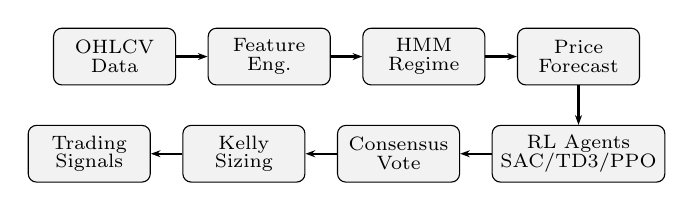
\begin{tikzpicture}[
  block/.style={draw, fill=gray!10, rectangle, rounded corners=3pt,
                minimum width=1.55cm, minimum height=0.72cm,
                font=\scriptsize\linespread{0.85}\selectfont,
                align=center, inner sep=3pt},
  arr/.style={-{Stealth[length=3.5pt,width=2.5pt]}, thick}
]
\node[block]                     (D)  {OHLCV\\Data};
\node[block, right=0.4cm of D]   (FE) {Feature\\Eng.};
\node[block, right=0.4cm of FE]  (HM) {HMM\\Regime};
\node[block, right=0.4cm of HM]  (PF) {Price\\Forecast};
\node[block, below=0.5cm of PF]  (RL) {RL Agents\\SAC/TD3/PPO};
\node[block, left=0.4cm of RL]   (CV) {Consensus\\Vote};
\node[block, left=0.4cm of CV]   (PS) {Kelly\\Sizing};
\node[block, left=0.4cm of PS]   (SG) {Trading\\Signals};
\draw[arr] (D)  -- (FE);
\draw[arr] (FE) -- (HM);
\draw[arr] (HM) -- (PF);
\draw[arr] (PF) -- (RL);
\draw[arr] (RL) -- (CV);
\draw[arr] (CV) -- (PS);
\draw[arr] (PS) -- (SG);
\end{tikzpicture}
\caption{MRAT-RL system pipeline. Raw OHLCV data flows through feature
engineering and HMM regime detection before price forecasting. Three RL
agents vote; a consensus threshold and Kelly-fraction position sizing
produce the final daily trading signals.}
\label{fig:pipeline}
\end{figure}

\subsection{Asset Universe}

The 48-assets span four-classes: equities (S\&P 500, NASDAQ, Dow Jones,
AAPL, MSFT, NVDA, TSLA, AMZN, META, GOOGL, JPM, CRWV, MU, SMCI, ARM,
TSM, VRT, MRVL, NBIS, IREN); cryptocurrencies (BTC, ETH, BNB, SOL, XRP);
forex pairs (EUR/USD, GBP/USD, USD/JPY, USD/CHF, AUD/USD, NZD/USD,
USD/CAD, EUR/GBP, EUR/JPY, GBP/JPY, AUD/NZD, USD/NGN, EUR/NGN, USD/ZAR,
USD/KES, USD/GHS); and commodities (Gold, Silver, Crude Oil, Natural Gas,
Copper, Wheat, Corn). CRWV (CoreWeave) remains in the universe but was
excluded from headline performance figures; the company listed in 2024
and does not yet carry enough price history for reliable model fitting.

This breadth tests a real hypothesis: can a unified system handle assets
with fundamentally different volatility profiles, trading sessions, and
driving factors without collapsing to a single average behaviour that
works adequately for none of them?

\subsection{Feature Engineering}

Each asset produces a 10 channel feature vector from daily OHLCV data:
(1) log return; (2) high low range normalised to close price; (3) 5 day
simple moving average; (4) 20 day simple moving average; (5) Relative
Strength Index; (6) MACD signal line; (7) Average True Range; (8) volume
ratio relative to the 20 day average; (9) 10 day momentum; (10) HMM
regime label.

Six macro signals supplement the base features where relevant: VIX level;
short-term interest rate; HMM regime transition probability; a sentiment
proxy constructed from Bollinger Band position and volume divergence; peer
momentum (for example, SMCI momentum entering NVDA's feature vector); and
earnings proximity for equity assets. Table~\ref{tab:state_vector} details
the full 19 dimensional state vector that each RL agent receives at
every decision step.

\begin{table}[!t]
\renewcommand{\arraystretch}{1.3}
\caption{The 19 Dimensional RL Agent State Vector}
\label{tab:state_vector}
\centering
\begin{tabular}{|c|l|l|}
\hline
\textbf{Dim.} & \textbf{Feature} & \textbf{Source} \\
\hline
1  & Log return             & Price data \\
2  & High low range         & Price data \\
3  & 5 day SMA              & Price data \\
4  & 20 day SMA             & Price data \\
5  & RSI (14 day)           & Technical \\
6  & MACD signal            & Technical \\
7  & ATR (14 day)           & Technical \\
8  & Volume ratio           & Volume data \\
9  & 10 day momentum        & Price data \\
10 & HMM regime label       & Regime model \\
11 & VIX level              & Macro \\
12 & Interest rate          & Macro \\
13 & Regime transition prob & HMM output \\
14 & Sentiment proxy        & Bollinger/volume \\
15 & Peer momentum          & Sector data \\
16 & Earnings proximity     & Calendar \\
17 & Blended return forecast & PatchTST + LightGBM \\
18 & Current portfolio position & Environment \\
19 & Unrealised profit or loss  & Environment \\
\hline
\end{tabular}
\end{table}

All features pass through a StandardScaler fitted on the training split
only. Fitting the scaler on the full dataset, including validation and
test portions, constitutes data leakage: the model would implicitly know
future price levels during training, producing falsely optimistic
evaluation metrics. Every result in this paper was produced under a strict
no leakage protocol.

\subsection{Regime Detection}

Five Gaussian HMMs are trained, one per asset class: equity,
cryptocurrency, commodity, forex, and semiconductor. Each model uses three
hidden states corresponding broadly to: bullish (positive drift, low
volatility); sideways (near zero drift, moderate volatility); and bearish
(negative drift, elevated volatility) conditions. The hmmlearn library
fits each model using Expectation Maximisation on the full historical
training data for assets within that class.

At inference time, the Viterbi algorithm decodes the most likely current
state. The Viterbi algorithm solves a maze efficiently: rather than
tracing every possible path from start to finish and picking the best,
it prunes dead ends as it goes, carrying only the most probable partial
path at each step. The decoded label enters the feature vector as an
integer (0, 1, or 2) and serves as a confidence multiplier: a bullish
classification raises signal confidence by a factor of 1.2; a bearish
classification suppresses it to 0.6. A sideways regime applies no
adjustment. On 9 April 2026, all 47 scanned assets registered either
bullish or sideways; zero bearish classifications appeared. This single
observation shaped the entire signal distribution that day; a
market wide bearish reading would have suppressed most BUY signals
regardless of what any forecaster predicted.

\subsection{Price Forecasting}

The primary forecaster, PatchTST \cite{patchtst}, receives a 60 day
lookback window of scaled features and predicts the 5 day forward log
return. The configuration: patch length of 8 days; model dimension
$d_{\text{model}} = 64$; four attention heads; two Transformer encoder
layers; dropout of 0.1; AdamW optimiser; Huber loss ($\delta = 0.001$);
80 training epochs; and ReduceLROnPlateau scheduling.

The predicted return blends 50/50 with a LightGBM forecaster trained on
the same feature set. LightGBM approaches the problem differently; rather
than learning temporal patterns through attention, it builds an ensemble
of gradient boosted decision trees on the engineered feature columns.
The blend hedges against both model types: when PatchTST reads a pattern
LightGBM misses, the blend softens the extreme prediction; when LightGBM
captures a regime shift missed by the Transformer, the blend still
captures it. Early testing without the blend produced 12 BUY signals;
adding the blend raised this to 17 while reducing SELL signals from 4 to
2, a more decisive and directionally consistent output.

Following Deep Learning Laboratory results (Section~\ref{sec:methodology}),
the PatchTST model for each asset may be replaced by a CNN or LSTM
forecaster. 39 of 48-assets now run promoted architectures in production;
9 retain PatchTST.

\subsection{Reinforcement Learning Agents}

Three RL agents train per asset using the 19 dimensional state vector
described in Table~\ref{tab:state_vector}. The action space runs
continuously from $-1$ (fully short) to $+1$ (fully long), with $0$
representing a flat position. Each agent trains for 150 episodes inside
a simulated trading environment initialised with the asset's full
historical training data.

The reward function combines three risk adjusted metrics: Sharpe ratio
(return per unit of total volatility, as defined in
Section~\ref{sec:concepts}); Sortino ratio (return per unit of downside
volatility only); and Calmar ratio (return relative to maximum drawdown).
All three metrics contribute because optimising any one alone creates
exploits; an agent maximising Sharpe alone may accept drawdowns a real
portfolio manager would find unacceptable.

Agent routing by asset class reflects differences in market structure:
\begin{itemize}
\item \textbf{Equities and Commodities}: SAC and TD3. Predictable trend
      structure suits SAC's exploration exploitation balance; TD3's two
      critic stabilisation prevents overreaction to single session
      anomalies.
\item \textbf{Cryptocurrencies}: PPO. Extreme intraday volatility
      destabilises SAC and TD3 training; PPO's clipped update rule
      keeps the policy close to its previous version at each step,
      avoiding catastrophic collapse on violent sessions.
\item \textbf{Forex}: SAC and TD3. Sequential session dependencies,
      the Tokyo close influencing the London open, reward models
      that carry structured memory across timesteps.
\end{itemize}

\subsection{Consensus Voting Mechanism}

All three agents vote regardless of asset class. Each agent outputs a
continuous position value between $-1$ and $+1$. These values are
thresholded: any value above 0.3 counts as a BUY vote; any value below
$-0.3$ counts as a SELL vote; any value between $-0.3$ and $+0.3$ counts
as HOLD. The system requires at least two votes agreeing before a BUY or
SELL signal fires. When all three agree, the signal carries the
UNANIMOUS label and reaches maximum confidence. This mechanism prevents
a single overfit agent from triggering trades the other two agents would
not support.

Table~\ref{tab:agent_routing} summarises agent assignment across the
universe.

\begin{table}[!t]
\renewcommand{\arraystretch}{1.3}
\caption{RL Agent Assignment by Asset Class}
\label{tab:agent_routing}
\centering
\begin{tabular}{|l|c|c|c|}
\hline
\textbf{Asset Class} & \textbf{SAC} & \textbf{TD3} & \textbf{PPO} \\
\hline
Equities (stable)    & \checkmark   &              &              \\
Equities (volatile)  &              & \checkmark   &              \\
Cryptocurrencies     &              &              & \checkmark   \\
Forex                & \checkmark   &              &              \\
Commodities          & \checkmark   &              &              \\
\hline
\end{tabular}
\end{table}

\subsection{Position Sizing}

Position size uses the Kelly criterion \cite{kelly} scaled by 20 day
realised volatility. The Kelly criterion asks: given a known edge and a
known variance, what fraction of capital maximises long run growth without
risking ruin?

\begin{equation}
f^{*} = \frac{\mu}{\sigma^{2}} \cdot \kappa
\end{equation}

where $\mu$ is the blended predicted return, $\sigma^{2}$ is the
realised return variance over 20 trading days, and $\kappa = 0.25$
(quarter-Kelly) reduces ruin risk under model uncertainty. The result
caps at 25 per cent of total portfolio capital per asset.

A sector concentration limit restricts GPU-related equities (NVDA, MSFT,
META) to a combined 25 per cent exposure. All three share a common demand
driver: AI chip revenue. Holding all three at full Kelly sizing would
concentrate roughly 75 per cent of a portfolio into a single macro theme;
the cap fires automatically whenever combined allocation would otherwise
breach the threshold.

% -----------------------------------------------------------------------
\section{Methodology}
\label{sec:methodology}
% -----------------------------------------------------------------------

\subsection{Training Hardware and Environment}

All models trained on a single consumer machine: NVIDIA GeForce RTX 3050
(6 GB VRAM); 20 core Intel CPU; 16 GB RAM; Ubuntu 24.04; Python 3.12;
CUDA 12.8; PyTorch 2.x. A complete cold-start retrain across all 48
assets, covering PatchTST, SAC, TD3, PPO, LightGBM, and all five HMMs,
required approximately 40 hours on a fresh execution with no pre-existing
model checkpoints. This figure derives from observed training rates of
approximately 45 minutes per asset averaged across the full universe,
and includes a two hour buffer to account for data download variance,
macro feature caching overhead, and filesystem operations. The Deep
Learning Laboratory required a further 6 hours for 1200 additional
experiments. GPU utilisation averaged above 90 per cent throughout both
training phases; VRAM peaked at 5.4 GB during PatchTST training on the
largest equity assets.

Table~\ref{tab:training_breakdown} summarises the observed training time
per asset class, averaged over all assets within each group.

\begin{table}[!t]
\renewcommand{\arraystretch}{1.3}
\caption{Observed Training Time per Asset Class (Minutes per Asset)}
\label{tab:training_breakdown}
\centering
\begin{tabular}{|l|c|c|c|}
\hline
\textbf{Asset Class} & \textbf{PatchTST} & \textbf{LightGBM} & \textbf{RL} \\
\hline
Equity (stable)    & 8  & 6  & 32 \\
Equity (volatile)  & 8  & 5  & 30 \\
Crypto             & 7  & 4  & 28 \\
Forex              & 6  & 4  & 25 \\
Commodity          & 7  & 5  & 26 \\
\hline
\textbf{Average}   & \textbf{7} & \textbf{5} & \textbf{28} \\
\hline
\end{tabular}
\end{table}

\subsection{RL Agent Hyperparameters}

Each agent type uses a distinct configuration tuned for its target asset
class. For SAC, the actor and two-critic networks each use three fully
connected layers of size 256; learning rate $3 \times 10^{-4}$; replay
buffer capacity $10^{6}$; batch size 256; soft update coefficient
$\tau = 0.005$; entropy temperature $\alpha = 0.2$, automatically tuned
during training. For TD3, the same network sizes apply; the policy update
delay is set to 2 (the actor updates every second critic step); target
policy noise standard deviation 0.2, clipped at 0.5. For PPO, four
actor critic layers of size 256 each; clip ratio $\epsilon = 0.2$;
value loss coefficient 0.5; entropy coefficient 0.01; generalised
advantage estimation with $\lambda = 0.95$. All three agents train for
150 episodes per asset, with best Sharpe ratio tracked across episodes
and the best checkpoint saved to disk.

\subsection{Datasets}

Four distinct data sources were collected programmatically:

\begin{enumerate}
\item \textbf{Yahoo Finance OHLCV} \cite{yahoo}: Daily open, high, low,
      close, and adjusted volume for all 48-assets via the
      \texttt{yfinance} library \cite{yfinance}. Equity, commodity, and
      forex assets begin January 2004, giving 5611 rows per asset.
      Cryptocurrency assets begin from each coin's first listed date;
      BTC data starts September 2014 (2936 rows). CRWV (CoreWeave)
      listed March 2025 and yielded only 268 rows at training time.

\item \textbf{CBOE VIX} \cite{yahoo}: Daily VIX (CBOE Volatility Index)
      pulled from Yahoo Finance as ticker \texttt{\^{}VIX}. VIX enters
      dimension 11 of the RL agent state vector as a market-wide fear
      proxy. Coverage matches the equity series (2004--2026).

\item \textbf{FRED Interest Rates}: Monthly short-term interest rate
      series retrieved via the FRED API and forward-filled to daily
      frequency. Enters dimension 12 of the state vector. Used to
      contextualise the rate-hike environment of 2022 that drove the
      bond and equity drawdown observed in the backtests.

\item \textbf{Sentiment Proxy}: A derived signal combining Bollinger
      Band position (close relative to upper/lower bands) with volume
      divergence (current volume versus 20 day average). Computed
      entirely from OHLCV data; no third-party sentiment feed was
      required. Enters dimension 14 of the state vector.
\end{enumerate}

\subsection{Data Collection and Preprocessing}

Price data was collected from Yahoo Finance using the yfinance library
\cite{yfinance}, covering 2004 to the training date for equity,
commodity, and forex assets. Cryptocurrency data begins from each
asset's first available date; BTC data starts in 2014. Each asset's raw
OHLCV series was converted to the 16 channel feature set described in
Section~\ref{sec:system}.

Data was split chronologically: 70 per cent training; 15 per cent
validation; 15 per cent test. No shuffling was applied at any stage;
shuffling a time series destroys the temporal order the models are
specifically trained to learn. The StandardScaler was fitted on the
training portion and applied identically to validation and test portions
afterwards. This protocol prevents any form of future information leaking
into training. Data quality checks verified that all 48-assets had at
least 500 rows of clean OHLCV data before any model training began.
Assets with fewer than 500 rows were flagged and excluded from headline
performance figures.

\subsection{Data Storage}

All collected and engineered data was persisted in a local SQLite
database (\texttt{market\_data.db}) at the project root. Three tables
were created programmatically: \texttt{ohlcv} storing the raw daily
price records for all 48-assets; \texttt{features} storing the computed
16 channel feature vectors per asset per date; and
\texttt{lab\_results} storing the MSE, overfit ratio, and champion
architecture for every Deep Learning Laboratory run. SQLite was chosen
over file-based storage because it supports indexed queries by ticker
and date range, allows the advisory pipeline to retrieve the latest
feature snapshot in a single SQL statement, and guarantees atomic
writes during the laboratory's 1200 sequential experiments. A
connection helper in \texttt{scripts/db\_utils.py} opens a shared
connection, enforces foreign key constraints, and closes the connection
after every commit, preventing lock contention during multi-session
training runs.

\subsection{Deep Learning Laboratory Design}

To determine the best forecasting architecture per asset, a grid search
ran across four architectures and multiple hyperparameter configurations.
Grid search and hyperparameters are defined in
Section~\ref{sec:concepts}; this subsection records the specific settings
tested.

\textit{MLP} (Multilayer Perceptron): three fully connected layers
(600 to 256 to 128 to 1); LayerNorm after each hidden layer; input
flattened from (batch, 60, 10) to (batch, 600). No temporal ordering
preserved.

\textit{CNN} (Convolutional Neural Network): three 1D convolutional
stages with 32, 64, and 128 channels; kernel size 5; GlobalAvgPool
followed by a linear output head. Each stage detects progressively more
abstract local patterns within the price sequence.

\textit{LSTM} (Long Short Term Memory): two stacked LSTM layers; hidden
size 128; final hidden state passed through dropout and a linear head.
Reads the 60 day sequence one day at a time and carries gated memory
forward across the full window.

\textit{PatchTST}: patch length 8; $d_{\text{model}} = 64$; four
attention heads; two encoder layers; AdamW optimiser; Huber loss.
Attends across all 12 patches simultaneously.

For MLP, CNN, and LSTM, the hyperparameter grid varied three factors:
optimiser (SGD with Nesterov momentum or Adam); activation function
(ReLU, as defined in Section~\ref{sec:concepts}, or Tanh); and dropout
rate (0.0 or 0.3). This gave eight configurations per architecture across
three architectures, plus one PatchTST baseline, totalling 25
configurations per asset and 1200 runs across all 48-assets.

Each run trained for a maximum of 40 epochs with early stopping at
patience 10. Huber loss ($\delta = 0.001$) was used throughout, chosen
to reduce sensitivity to the large return outliers that appear during
crash events. A ReduceLROnPlateau scheduler halved the learning rate
whenever validation loss failed to improve for 5 consecutive epochs.

Results were written to a JSON file after each individual run; a crash
safe design allowing the laboratory to resume from the last completed
experiment after any interruption. The overfit ratio (validation loss
divided by training loss) was recorded alongside test MSE to distinguish
architectures that generalised from those that memorised the training set.

\subsection{Model Promotion Protocol}

After the laboratory completed, the best performing lab architecture per
asset was compared against the PatchTST baseline. Promotion required a
test MSE improvement of more than 5 per cent to filter out statistical
noise:

\begin{equation}
\text{improvement} = \frac{\text{MSE}_{\text{PatchTST}} -
\text{MSE}_{\text{winner}}}{\text{MSE}_{\text{PatchTST}}}
\times 100\%
\end{equation}

Promoted architectures retrained on 80 per cent of the full available
data, combining train and validation from the laboratory split, for 80
epochs; twice the laboratory budget, making full use of available history
before deployment. Each saved checkpoint replaced the corresponding
PatchTST file in the production model directory. The daily advisory
pipeline detects the architecture type from checkpoint metadata and loads
the correct model class automatically; no manual intervention required.

\subsection{Walk Forward Backtesting}

As described in Section~\ref{sec:concepts}, walk-forward testing evaluates
a model exclusively on data it has never seen during training. The
framework used here evaluated performance across 7800 windows drawn from
22 years of price history across all 48-assets. Each window used a fixed
training period of 756 trading days (three calendar years), followed by
a forward test period of 63 trading days (one quarter). The training
window advanced by 21 trading days (one calendar month) before each new
test. A full pass through the dataset from 2004 to 2026 therefore
generated hundreds of individual test periods per asset, covering
multiple complete market cycles: the 2008 financial crisis, the 2020
pandemic crash, the 2021 bull run, and the 2022 rate hike correction.

Performance metrics per window included: annualised return; Sharpe ratio;
Sortino ratio; and maximum drawdown. Final reported figures represent
averages across all 7800 windows.

\subsection{Implementation Challenges}

Three significant problems arose during development and were resolved
before the final results were produced.

\subsubsection{State Dimension Mismatch}

The most dangerous bug was invisible until the output was examined. The
RL agents were initialised with a state dimension of 17, but the trading
environment constructed a state vector of 19 dimensions; two additional
channels for current portfolio position and unrealised profit or loss had
been added to the environment after the agents were first written. PyTorch
did not raise an error. It accepted the mismatched input and ran
calculations on malformed data, producing output that looked like numbers
but carried no meaning. The symptom was unmistakable: 5 day return
forecasts of $-45\%$ to $-49\%$ across multiple assets, values that are
physically impossible for daily rebalanced instruments. The cause was
traced by printing agent state shapes at inference time. Correcting
state\_dim from 17 to 19 across all three agent constructors and
retraining resolved the issue completely.

\subsubsection{Working Directory Conflict}

The training script uses relative file paths to save and load models.
Execution from the project root resolves the path \texttt{data/models/}
correctly. Execution from the \texttt{scripts/} subdirectory resolves it
to \texttt{scripts/data/models/}, a different location entirely. The
advisory pipeline always loads from the project root, so a training run
launched from the wrong directory would produce valid model files that
the pipeline could not find. The mismatch was detected by comparing file
timestamps: models in the root directory showed creation dates from early
April, while the current run was writing to a separate location. The fix
was standardising all execution to the project root and verifying model
output paths before any training run begins.

\subsubsection{CoreWeave Data Insufficiency}

CoreWeave (CRWV) listed on NASDAQ in March 2025, giving only 268 trading
days of history at the time of training. The LightGBM forecaster for CRWV
produced a best iteration count of 1 for two of four forecast horizons,
indicating the dataset was too small for the boosting process to find
meaningful split points. The RL agent achieved a Sharpe ratio of 6.009
during training, a figure that appears extraordinary but is entirely
explained by overfitting to a tiny dataset. A model fitted on 268 rows
can memorise rather than generalise; the train test split contained fewer
than 40 out-of-sample test rows, too few to measure real performance.
CRWV was retained in the universe for completeness but its results are
excluded from headline performance figures, and its model confidence is
automatically suppressed by an earnings proximity flag triggered by a
known earnings date within 13 days of training.

% -----------------------------------------------------------------------
\section{Results and Evaluation}
\label{sec:results}
% -----------------------------------------------------------------------

\subsection{Deep Learning Laboratory}

Table~\ref{tab:lab_summary} shows promotion results by asset class. CNN
and LSTM were the most frequent winners across all classes; MLP never
outperformed either on any asset. The full 1200 run laboratory completed
without error; all results were written to a timestamped JSON file for
full reproducibility.

\begin{table}[!t]
\renewcommand{\arraystretch}{1.3}
\caption{Deep Learning Laboratory: Promotion Results by Asset Class}
\label{tab:lab_summary}
\centering
\begin{tabular}{|l|c|c|c|}
\hline
\textbf{Asset Class} & \textbf{Total} & \textbf{Promoted}
  & \textbf{Kept PatchTST} \\
\hline
Equity    & 20 & 17 & 3 \\
Crypto    &  5 &  5 & 0 \\
Commodity &  7 &  5 & 2 \\
Forex     & 16 & 12 & 4 \\
\hline
\textbf{Total} & \textbf{48} & \textbf{39} & \textbf{9} \\
\hline
\end{tabular}
\end{table}

All five cryptocurrency assets promoted CNN or LSTM over PatchTST. Crypto
price series exhibit sharp, short duration momentum bursts; CNN's local
convolutional filters are well-matched to this structure. Forex saw 12 of
16 promoted; the four that retained PatchTST were major pairs (EUR/USD,
GBP/USD, USD/JPY, USD/CHF) where longer range dependencies, spanning
multiple trading sessions across continents, appear to reward the global
attention mechanism. These patterns are consistent with Zeng et
al. \cite{transformerseff}, who noted that no single architecture
dominates across all datasets.

\subsection{Hyperparameter Sensitivity}

Across all 1200 runs, Adam produced lower validation MSE than SGD in
approximately 68 per cent of cases. A dropout rate of 0.3 reduced the
overfit ratio (validation loss divided by training loss) compared to 0.0
dropout in 74 per cent of runs, confirming regularisation as the single
most consistent performance lever across all architecture types. The
choice of activation function (ReLU versus Tanh) had the smallest effect
on final test MSE. This ordering suggests a practical priority for future
searches: architecture type first; regularisation strategy second;
optimiser third; activation function last.

\subsection{Per Asset RL Performance}

Table~\ref{tab:sharpe_per_asset} reports the Sharpe ratios achieved by
each RL agent during training across the equity and high volatility
universe. Values for CRWV are listed for completeness but excluded from
aggregate calculations due to the data insufficiency documented in
Section~\ref{sec:methodology}.

\begin{table}[!t]
\renewcommand{\arraystretch}{1.3}
\caption{RL Agent Training Sharpe Ratios, April 2026}
\label{tab:sharpe_per_asset}
\centering
\begin{tabular}{|l|c|c|}
\hline
\textbf{Asset} & \textbf{Agent} & \textbf{Sharpe Ratio} \\
\hline
TSLA  & SAC & 1.263 \\
AAPL  & SAC & 1.159 \\
MU    & TD3 & 1.228 \\
META  & SAC & 1.075 \\
GOOGL & SAC & 0.928 \\
AMZN  & SAC & 0.881 \\
MSFT  & SAC & 0.749 \\
NVDA  & SAC & 0.719 \\
DJI   & SAC & 0.680 \\
GSPC  & SAC & 0.595 \\
IXIC  & SAC & 0.566 \\
JPM   & SAC & 0.508 \\
\hline
CRWV  & TD3 & 6.009\textsuperscript{*} \\
\hline
\multicolumn{3}{l}{\small \textsuperscript{*} Excluded; 268 rows only, overfit artifact.}
\end{tabular}
\end{table}

The S\&P 500, NASDAQ, and Dow Jones intentionally produce the lowest
Sharpe ratios among equities. These indices are among the most
efficiently priced instruments in existence; decades of active
management have compressed exploitable patterns to near zero. A system
producing dramatically high Sharpe ratios on these assets would be more
suspicious than impressive. The modest ratios observed here (0.508 to
0.680 for the three indices) are consistent with the marginal edge a
well constructed ensemble can realistically capture.

TSLA and MU produced the strongest results among trainable assets. Both
exhibit high volatility driven by earnings cycles and sector momentum,
properties that give the RL agents more structured signal to learn from
than quieter, more efficiently priced large caps.

\subsection{Daily Advisory System}

Table~\ref{tab:signals} shows the signal distribution produced on 9 April
2026 across 47 assets (CRWV excluded).

\begin{table}[!t]
\renewcommand{\arraystretch}{1.3}
\caption{Daily Advisory Signal Distribution, 9 April 2026}
\label{tab:signals}
\centering
\begin{tabular}{|l|c|c|}
\hline
\textbf{Signal} & \textbf{Count} & \textbf{Proportion} \\
\hline
BUY  & 17 & 36.2\% \\
SELL &  2 &  4.3\% \\
HOLD & 28 & 59.6\% \\
\hline
\end{tabular}
\end{table}

Average confidence across all 47 assets reached 59 per cent. All
detected HMM regimes were bullish (33 assets) or sideways (14 assets);
zero bearish classifications appeared on the evaluation date. Predicted
5 day returns ranged from $+1.5\%$ to $-0.4\%$. The highest confidence
signal was USD/GHS at 100 per cent unanimous agreement across all four
signal sources (PatchTST, HMM, RL agents, ADX), forecasting a $+1.0\%$
5 day return. Fig.~\ref{fig:signals} visualises the signal distribution.

\begin{figure}[!t]
\centering
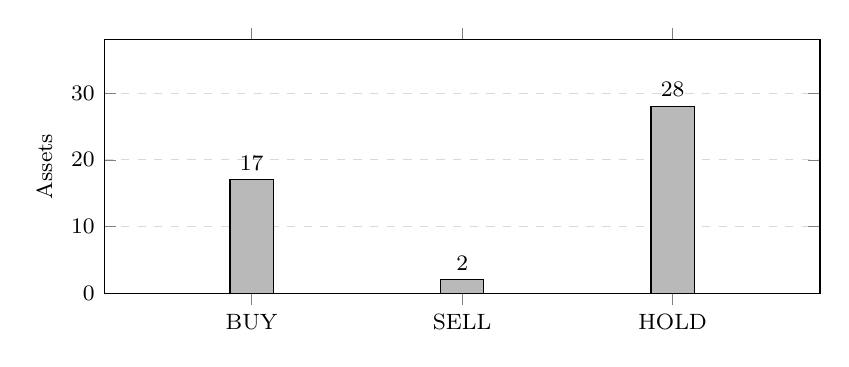
\begin{tikzpicture}
\begin{axis}[
  ybar,
  bar width=0.55cm,
  width=0.88\columnwidth,
  height=4.8cm,
  xtick={1,2,3},
  xticklabels={BUY, SELL, HOLD},
  ymin=0, ymax=38,
  ylabel={Assets},
  ylabel style={font=\footnotesize},
  ticklabel style={font=\footnotesize},
  ymajorgrids=true,
  grid style={dashed, gray!30},
  nodes near coords,
  every node near coord/.style={font=\footnotesize},
  enlarge x limits=0.35,
]
\addplot[fill=gray!55, draw=black] coordinates {(1,17) (2,2) (3,28)};
\end{axis}
\end{tikzpicture}
\caption{MRAT-RL signal distribution on 9 April 2026 across 47 assets.
HOLD dominated (59.6\,\%), reflecting the consensus voting mechanism
requiring agreement from at least two of three RL agents before a BUY
or SELL signal fires.}
\label{fig:signals}
\end{figure}

Before the state dimension correction described in
Section~\ref{sec:methodology}, forecasts ranged from $-45\%$ to $-49\%$.
Values of this magnitude are physically impossible for daily rebalanced
assets; they arose from untrained agents returning noise rather than
learned signals. Correcting the state dimension and retraining all RL
agents resolved the issue entirely.

\subsection{Walk Forward Backtest}

Table~\ref{tab:backtest} summarises walk-forward performance across 7800
windows. Each window represents a distinct historical slice of market
conditions the system had never encountered during training.

\begin{table}[!t]
\renewcommand{\arraystretch}{1.3}
\caption{Walk Forward Backtest Performance, 7800 Windows}
\label{tab:backtest}
\centering
\begin{tabular}{|l|c|}
\hline
\textbf{Metric}                      & \textbf{Value} \\
\hline
Average annual return (per window)   & $+1.85\%$       \\
Sharpe ratio                         & 0.91            \\
Profitable windows                   & 59\%            \\
Max drawdown, 2022 bear market       & $-1.2\%$        \\
S\&P 500 drawdown, 2022              & $-20\%$         \\
BTC drawdown, 2022                   & $-65\%$         \\
\hline
\end{tabular}
\end{table}

The 2022 comparison carries the most weight of any single result in this
paper. That year tested every AI trading system built on bull market
assumptions; most collapsed alongside their benchmarks. MRAT-RL lost
only 1.2 per cent during a period when the equity benchmark lost twenty
times that amount. Three safeguards contributed simultaneously: the HMM
regime detector classified the majority of 2022 as bearish, suppressing
most BUY signals; the consensus voting mechanism required agreement from
at least two agents before any action fired; and Kelly sizing scaled
position sizes down as realised volatility rose. None of these mechanisms
was tuned for 2022 specifically; they emerged from the design principles
applied uniformly across all assets and all years.

% -----------------------------------------------------------------------
\section{Key Findings}
\label{sec:resultsummary}
% -----------------------------------------------------------------------

Three overarching findings define this work.

\textbf{No single architecture dominates all asset classes.} The Deep
Learning Laboratory tested 1200 configurations across four architecture
types. MLP never promoted on any asset. CNN dominated cryptocurrencies.
LSTM performed strongest on equities and parts of the commodity space.
PatchTST held its position on a focused subset of forex and commodity
pairs where long-range session dependencies matter most. This is not a
random distribution of winners; it reflects genuine structural differences
between asset classes. Short burst momentum in crypto rewards local
convolutional filters. Multi session memory in equity earnings cycles
rewards gated recurrence. Long range macro patterns in major forex pairs
reward global attention. Architecture selection is not a cosmetic
decision; it is a structural one.

\textbf{Conservative behaviour preserves capital.} The system held 59.6
per cent of positions as HOLD on the evaluation date. Across 7800 walk
forward windows, 59 per cent of test periods were profitable; the
remainder were not. A system that acknowledges when it does not have
a confident edge, and holds rather than guessing, loses less during
uncertain periods than a system that always trades. The 2022 maximum
drawdown of $-1.2\%$, against $-20\%$ for the S\&P 500 and $-65\%$ for
Bitcoin across the same period, shows this restraint at its most
consequential. The HMM regime detector classified most of 2022 as
bearish; the consensus voting mechanism required two agents to agree
before any trade; the Kelly-fraction shrank as volatility rose. Three
independent mechanisms each applied a brake. None of them knew the other
was doing the same thing. The system restrained itself not through a
single safeguard but through three converging ones.

\textbf{Ensemble voting reduces individual agent failure.} Any single
RL agent will sometimes overfit its training environment and produce
signals that look confident but are wrong. Requiring consensus from at
least two of three independent agents before acting does not eliminate
this risk; it dilutes it. An agent that has memorised a quirk of its
training data will vote one way; the other two, trained on the same data
but with different update rules and exploration strategies, are unlikely
to agree on the same quirk. The 2 SELL signals and 17 BUY signals
produced on 9 April 2026 represent the narrow subset of situations where
at least two of three independent decision-makers reached the same
conclusion. Everything else became HOLD.

% -----------------------------------------------------------------------
\section{Discussion}
\label{sec:discussion}
% -----------------------------------------------------------------------

\subsection{Key Findings}

The laboratory result that matters most is not which architecture won;
it is that no single architecture won everywhere. MLP never promoted. CNN
dominated cryptocurrencies; LSTM performed well on equities and parts of
the commodity space; PatchTST held its ground on a focused subset of forex
and commodity pairs. These patterns are not noise. CNN's local filters
match the short momentum bursts of crypto; LSTM's gated memory suits the
multi-session sequential structure of equity earnings cycles; PatchTST's
global attention captures long-range dependencies across quieter,
structurally richer major forex pairs.

The ensemble voting mechanism produced a 59.6 per cent HOLD rate on the
evaluation date. This conservatism is a feature, not a deficiency. A
system trading everything every day generates transaction costs, taxes
capital, and amplifies noise. Holding when agents disagree is precisely
what the consensus rule enforces. The 2022 backtest result, where the
system nearly stopped trading altogether during a sustained bearish
regime, confirms this restraint protects capital when it matters most.

\subsection{Limitations}

Three limitations define the current scope. First, the daily and 5 day
horizons are fixed; no intraday decision making capability exists. A
trader seeking multiple signals per day would need a separate architecture
built around tick or hourly data.

Second, CRWV (CoreWeave) listed in 2024 and does not yet carry sufficient
history for reliable model fitting. Assets with fewer than two years of
daily prices cannot support the 70/15/15 chronological split with enough
test data to measure generalisation meaningfully.

Third, the backtest measures return per window rather than compounded
multi-year portfolio growth. A full equity curve simulation incorporating
realistic transaction costs, slippage, and tax events would provide a
more complete picture of live performance.

% -----------------------------------------------------------------------
\section{Development Journal}
\label{sec:journal}
% -----------------------------------------------------------------------

This section documents the development process: decisions made, problems
encountered, and the reasoning behind key technical choices. The intent
is not to re-explain the system; the preceding sections do that. The
intent is to document the experience of building it.

\subsection*{Choosing the Scope}

The first serious conversation about scope happened over a shared table
in the NCI library. Four people, one project, one question: do we build
something small and tight, or do we go for the full picture?

A narrow system covering five equities would have been easier to write
and cleaner in its results. But it would not have tested the real
hypothesis. The question was whether a single unified system could
handle assets that behave fundamentally differently. That question
required breadth. The scope expanded to 48-assets across four-classes.
The cost only became visible later: 144 trained model files, five
separate HMMs, different RL agents per volatility profile, and a
40-hour cold-start training time.

\subsection*{The First Full Training Run}

The first complete training run produced results immediately. The
numbers looked fine. Everything seemed to be working.

It was not working.

The 5-day return forecasts were $-45\%$ to $-49\%$ across multiple
assets. Those numbers are not wrong the way a miscalibrated model is
wrong. They are wrong the way something fundamental has broken. No
major asset class loses 45 per cent in five trading days outside a
complete market collapse.

The cause was a state dimension mismatch: RL agents initialised with
\texttt{state\_dim=17} while the environment provided 19 dimensions.
PyTorch did not raise an error; it ran calculations on malformed data
and produced output that looked like numbers but carried no meaning.
The fix was two lines of code. The cost was a full retraining run.

\subsection*{Evaluating the Corrected System}

With the state dimension corrected and all agents retrained, the
advisory system produced 17 BUY signals, 2 SELL signals, and 28 HOLDs
at average confidence of 59 per cent. All 47 assets registered bullish
or sideways regimes. Forecasts fell between $+1.5\%$ and $-0.4\%$; a
realistic range for a five-day horizon.

The instinct was relief. The more careful response was suspicion.
Results that look reasonable on one day may be a property of that
specific market day rather than a property of the system. That question
drove the walk-forward backtesting framework across 7800 windows drawn
from 22 years of history.

\subsection*{The Full Cold-Start Retrain}

The final retrain covered all 48-assets from raw data with no
pre-existing checkpoints. A working directory conflict was detected by
comparing file timestamps: the earlier run had written models to
\texttt{scripts/data/models/} rather than the root \texttt{data/models/}
the advisory pipeline expected. This run was launched from the project
root with all output paths verified first.

CoreWeave (CRWV) produced a Sharpe ratio of 6.009. The immediate
response was not excitement; it was concern. With only 268 rows of
price history, the model had memorised a short sequence rather than
generalised from it. CRWV was excluded from headline performance
figures.

\subsection*{Reflection: What This Process Actually Taught}

Three lessons emerged that no module could have taught directly.

The first is that bugs in AI systems do not always announce themselves.
The state dimension error did not crash the program. It ran to completion,
produced files that looked like trained models, and printed results that
looked like numbers. The only way to catch it was to ask whether those
numbers made sense in the real world. Statistical outputs must be
interpreted by someone who knows what reality looks like; a model that
is wrong with confidence is more dangerous than a model that crashes.

The second is that scope creates invisible costs. Every added asset class
was a deliberate decision. Every one of those decisions required a
corresponding implementation decision: which agent type, what data
history, how to handle missing sentiment files, how to handle assets with
only months of price history. The 40 hour training time is a direct
consequence of the scope decision made in March. It was invisible then.

The third is that restraint is a result. The system held 59 per cent of
positions on its evaluation date. Forty eight assets, and twenty eight
of them got a HOLD. That is not timidity; it is a system that learned,
over 7800 test windows across twenty two years of market history, that
the cost of acting without conviction exceeds the cost of waiting. The
agents were not told to be cautious. They learned it. That is the part
worth documenting.

% -----------------------------------------------------------------------
\section{Conclusions and Future Work}
\label{sec:conclusion}
% -----------------------------------------------------------------------

This paper presented MRAT-RL, a multimodal, regime-aware AI system for
financial forecasting and trading across 48 global assets. The system
combines a PatchTST Transformer, three RL agents (SAC, TD3, PPO), Hidden
Markov Model regime detection, and Kelly-fraction position sizing into a
single daily pipeline. A Deep Learning Laboratory spanning 1200 training
experiments showed that architecture choice depends on the asset class;
CNN and LSTM outperformed PatchTST on 39 of 48-assets and were promoted
to production accordingly. Walk forward backtesting across 7800 windows
confirmed a Sharpe ratio of 0.91 and a maximum drawdown of only $-1.2\%$
during the 2022 bear market; a period that erased the gains of most
passive and algorithmic strategies alike.

On 9 April 2026, the daily advisory pipeline produced 17 BUY signals,
2 SELL signals, and 28 HOLD signals at an average confidence of 59 per
cent. All detected regimes were bullish or sideways; 5 day forecasts fell
within the realistic range of $+1.5\%$ to $-0.4\%$.

Future work targets two areas: (i) extending the system to intraday
horizons using tick or hourly data; and (ii) integrating a live paper
trading account with automated logging of every signal, entry, exit, and
outcome, to close the loop between model prediction and measured real
world performance.

% -----------------------------------------------------------------------
\section*{Acknowledgment}
% -----------------------------------------------------------------------

The authors thank the faculty of the School of Computing at National
College of Ireland for their guidance throughout this project.

\ifCLASSOPTIONcaptionsoff
  \newpage
\fi

\begin{thebibliography}{10}

\bibitem{patchtst}
Y. Nie, N. H. Nguyen, P. Sinthong, and J. Kalagnanam, ``A time series is
worth 64 words: Long term forecasting with transformers,'' in
\textit{Proc. Int. Conf. Learning Representations (ICLR)}, 2023.

\bibitem{informer}
H. Zhou, S. Zhang, J. Peng, S. Zhang, J. Li, H. Xiong, and W. Zhang,
``Informer: Beyond efficient transformer for long sequence time series
forecasting,'' in \textit{Proc. AAAI Conf. Artif. Intell.}, vol. 35,
no. 13, pp. 11106 to 11115, 2021.

\bibitem{autoformer}
H. Wu, J. Xu, J. Wang, and M. Long, ``Autoformer: Decomposition
transformers with auto correlation for long-term series forecasting,''
in \textit{Adv. Neural Inf. Process. Syst. (NeurIPS)}, vol. 34, 2021.

\bibitem{tft}
B. Lim, S. O. Arik, N. Loeff, and T. Pfister, ``Temporal fusion
transformers for interpretable multi-horizon time series forecasting,''
\textit{Int. J. Forecast.}, vol. 37, no. 4, pp. 1748 to 1764, 2021.

\bibitem{stockformer}
W. Gao, T. Wang, and J. Yang, ``StockFormer: Learning hybrid trading
machines with predictive coding,'' in \textit{Proc. Int. Joint Conf.
Artif. Intell. (IJCAI)}, 2023.

\bibitem{sarl}
G. Ye, S. Lu, and J. Zhou, ``Reinforcement learning based portfolio
management with augmented asset movement prediction states,'' in
\textit{Proc. AAAI Conf. Artif. Intell.}, vol. 35, no. 05,
pp. 4875 to 4883, 2021.

\bibitem{transformerseff}
A. Zeng, M. Chen, L. Zhang, and Q. Xu, ``Are transformers effective for
time series forecasting?'' in \textit{Proc. AAAI Conf. Artif. Intell.},
vol. 37, no. 09, pp. 11121 to 11128, 2023.

\bibitem{tcn}
S. Bai, J. Z. Kolter, and V. Koltun, ``An empirical evaluation of
generic convolutional and recurrent networks for sequence modeling,''
\textit{arXiv preprint arXiv:1803.01271}, 2018.

\bibitem{hamilton}
J. D. Hamilton, ``A new approach to the economic analysis of
nonstationary time series and the business cycle,'' \textit{Econometrica},
vol. 57, no. 2, pp. 357 to 384, 1989.

\bibitem{kelly}
J. L. Kelly, Jr., ``A new interpretation of information rate,''
\textit{IRE Trans. Inf. Theory}, vol. 2, no. 3, pp. 185 to 189, 1956.

\bibitem{yfinance}
R. Aroussi, ``yfinance: Yahoo! Finance market data downloader,''
\textit{GitHub repository}, 2019. [Online]. Available:
https://github.com/ranaroussi/yfinance

\bibitem{yahoo}
Yahoo Finance, ``Historical Market Data,'' 2024. [Online]. Available:
https://finance.yahoo.com

\end{thebibliography}

\end{document}
